\documentclass{article}
\usepackage{hyperref}
\usepackage{graphicx} % Required for inserting images

\title{Plan}
\author{Automatic Project Detection And Tooling For Devs}
\date{}

\begin{document}
\maketitle

\section{Full work breakdown}

\section{Tasks}

\section{Structure of tasks}

\section{Task assignment}

\section{Time management}

\newpage
\section{Architecture}

\subsection{Software components}

The program is built on three main layers, each representing a namespace. These are:
\begin{itemize}
    \item Model: handles the business logic. Finds runnables, and collects its details. Executes the runnables.
    \item Persistence: handles the IO operations. Saves and loads user preferences and other information that is needed for better usability.
    \item View: stands for the user interface.
\end{itemize}

The following image shows the structure of the 3 layer, and all files in the layers. 

\begin{figure}[h]
    \centering
    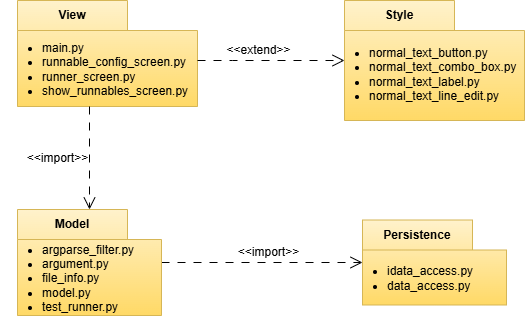
\includegraphics[width=1\linewidth]{img/package_diagram.drawio.png}
    \caption{UML package diagram}
    \label{fig:enter-label}
\end{figure}

The UML class diagram of Model and Persistence layers shows the structure of each objects and the relations between each other.

\begin{figure}[h]
    \centering
    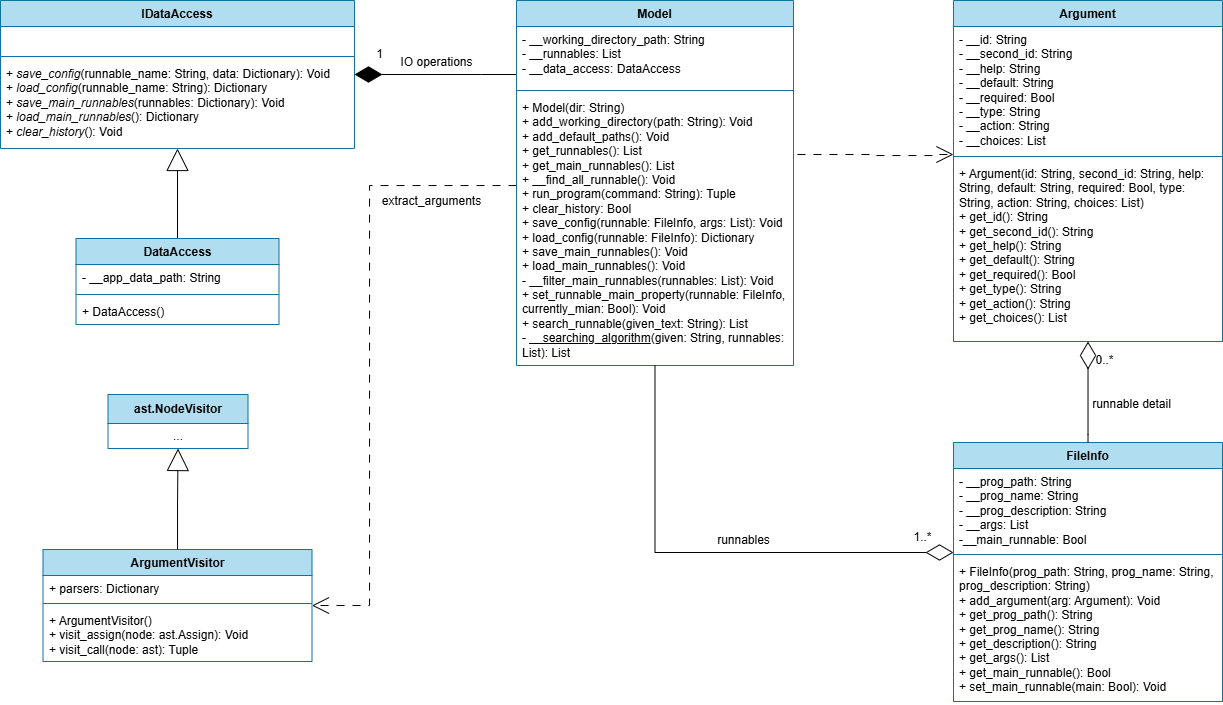
\includegraphics[width=1\linewidth]{img/class_diagram_model_persistence.drawio.png}
    \caption{UML class diagram of Model and Persistence layers}
    \label{fig:enter-label}
\end{figure}

The UML class diagram of View layer shows the structure of each objects and the relations between each other.

\begin{figure}[h]
    \centering
    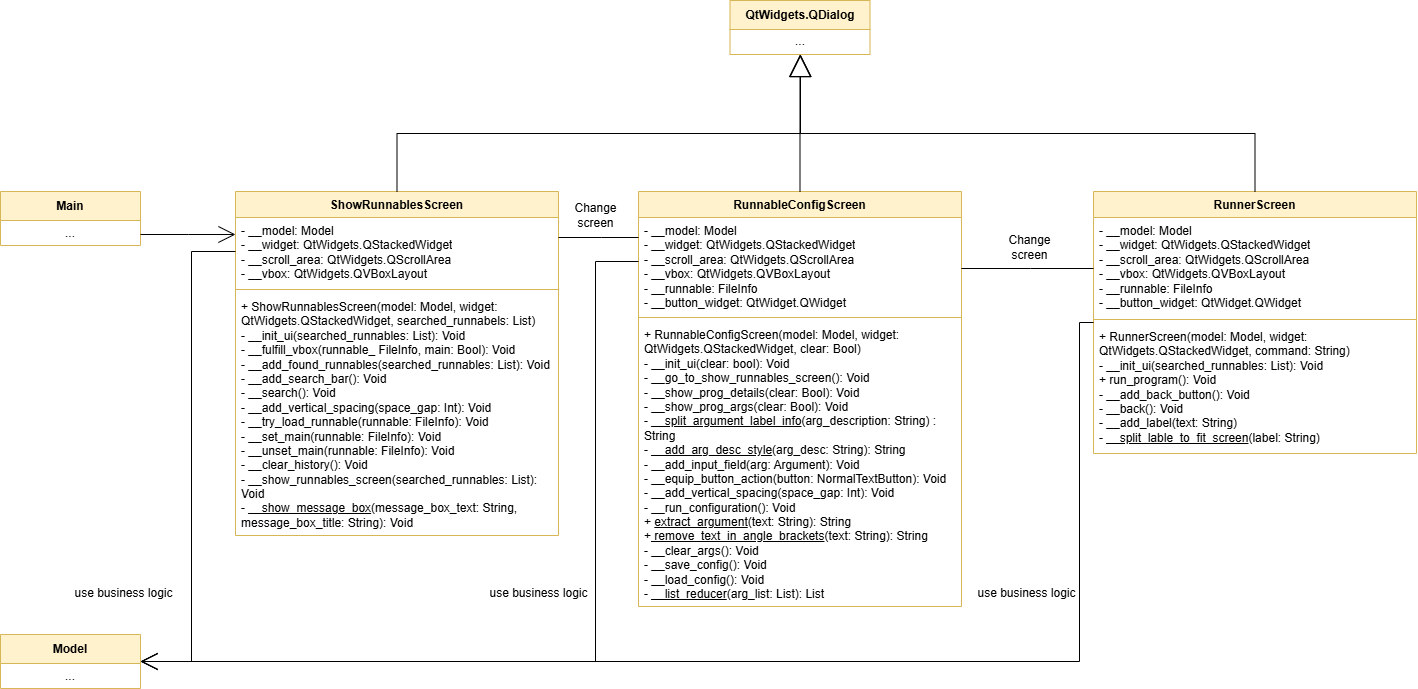
\includegraphics[width=1\linewidth]{img/class_diagram_view.drawio.png}
    \caption{UML class diagram of View layer}
    \label{fig:enter-label}
\end{figure}

The View has 3 screens.
\begin{itemize}
    \item The first one shows all the executables. An executable can be reached with a button. Every executable can be pinned as favourite. The screen also contains a search bar and a clear history button.
    \item The second screen shows an executable all information. Lists all the arguments and offers an opportunity to give a value to it. The user can also run the program here.
    \item The third and last screen shows the output messages, logs or errors for the user, after a program execution.
\end{itemize}
The screens' wire frame plan can be seen below.

\begin{figure}[h]
    \centering
    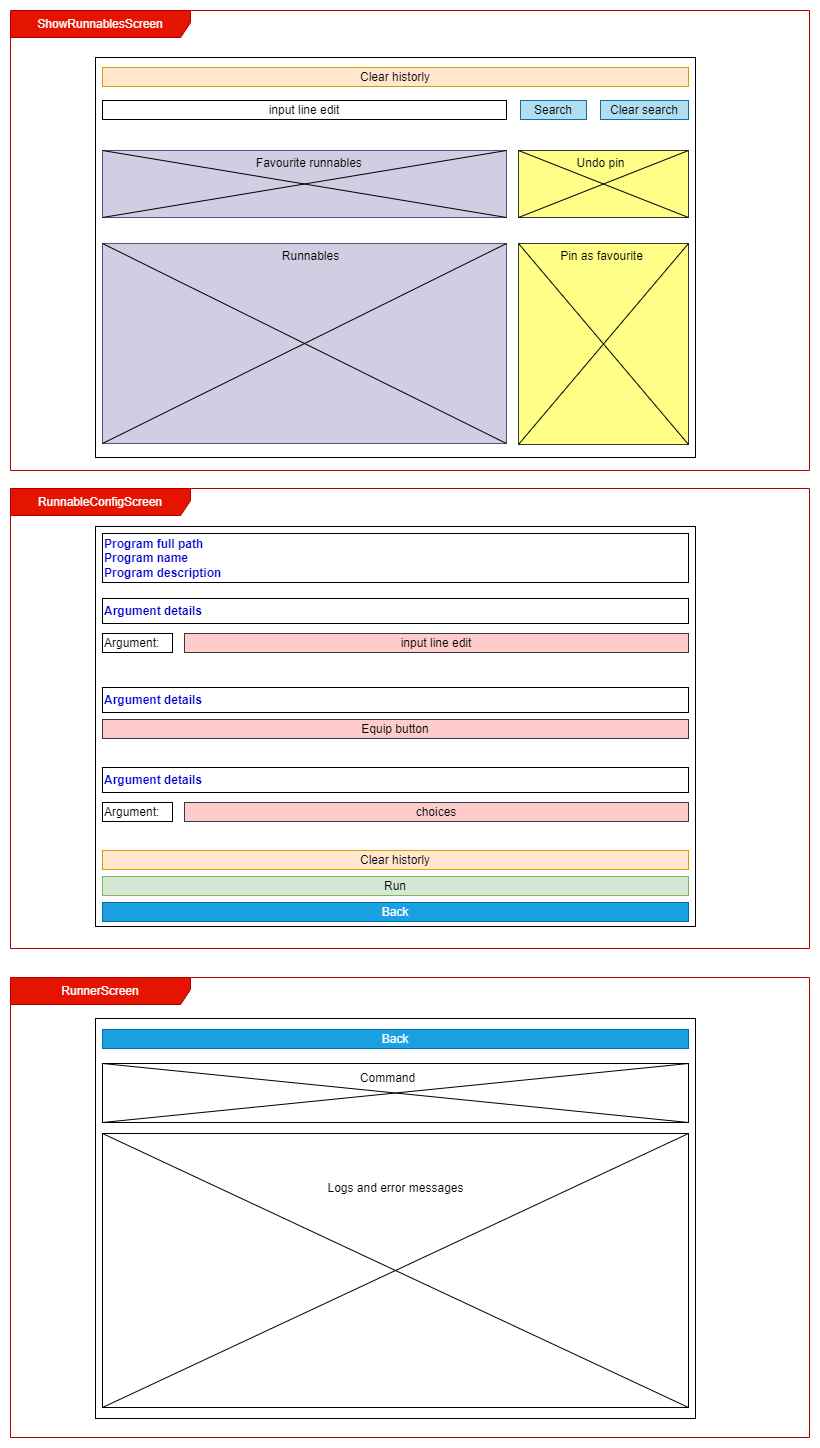
\includegraphics[width=1\linewidth]{img/wire_frame_plan.drawio.png}
    \caption{Screens' wire frame plan}
    \label{fig:enter-label}
\end{figure}

\newpage

\subsection{Software installation}
To install the software, follow these steps:
\begin{enumerate}
    \item Clone the repository: \texttt{git clone <repo\_url>}.
    \item Install dependencies: Run \texttt{npm install} (for Node.js environment) or \texttt{pip install -r requirements.txt} (for Python).
    \item Start the application: \texttt{npm start} or \texttt{python app.py}.
\end{enumerate}

\subsection{Software requirements}
The following tools and environments are required:
\begin{itemize}
    \item Operating System: Windows/Linux/MacOS
    \item Programming Language: Node.js or Python (v3.8+)
    \item Additional dependencies: Docker, PostgreSQL (if applicable)
    \item Disk space: At least 500MB of free space
    \item RAM: 4GB minimum (recommended 8GB for better performance)
\end{itemize}



\end{document}
